\chapter{Endometrial Biopsy}

\section*{Overview}
An endometrial biopsy takes a small sample from the lining of the uterus (the endometrium). A laboratory examines the tissue under a microscope. The test can help find causes of abnormal uterine bleeding and detect conditions such as endometrial hyperplasia or cancer. It does not by itself show every structural cause of bleeding, such as a polyp.


\begin{center}
\begin{minipage}{\textwidth}\centering
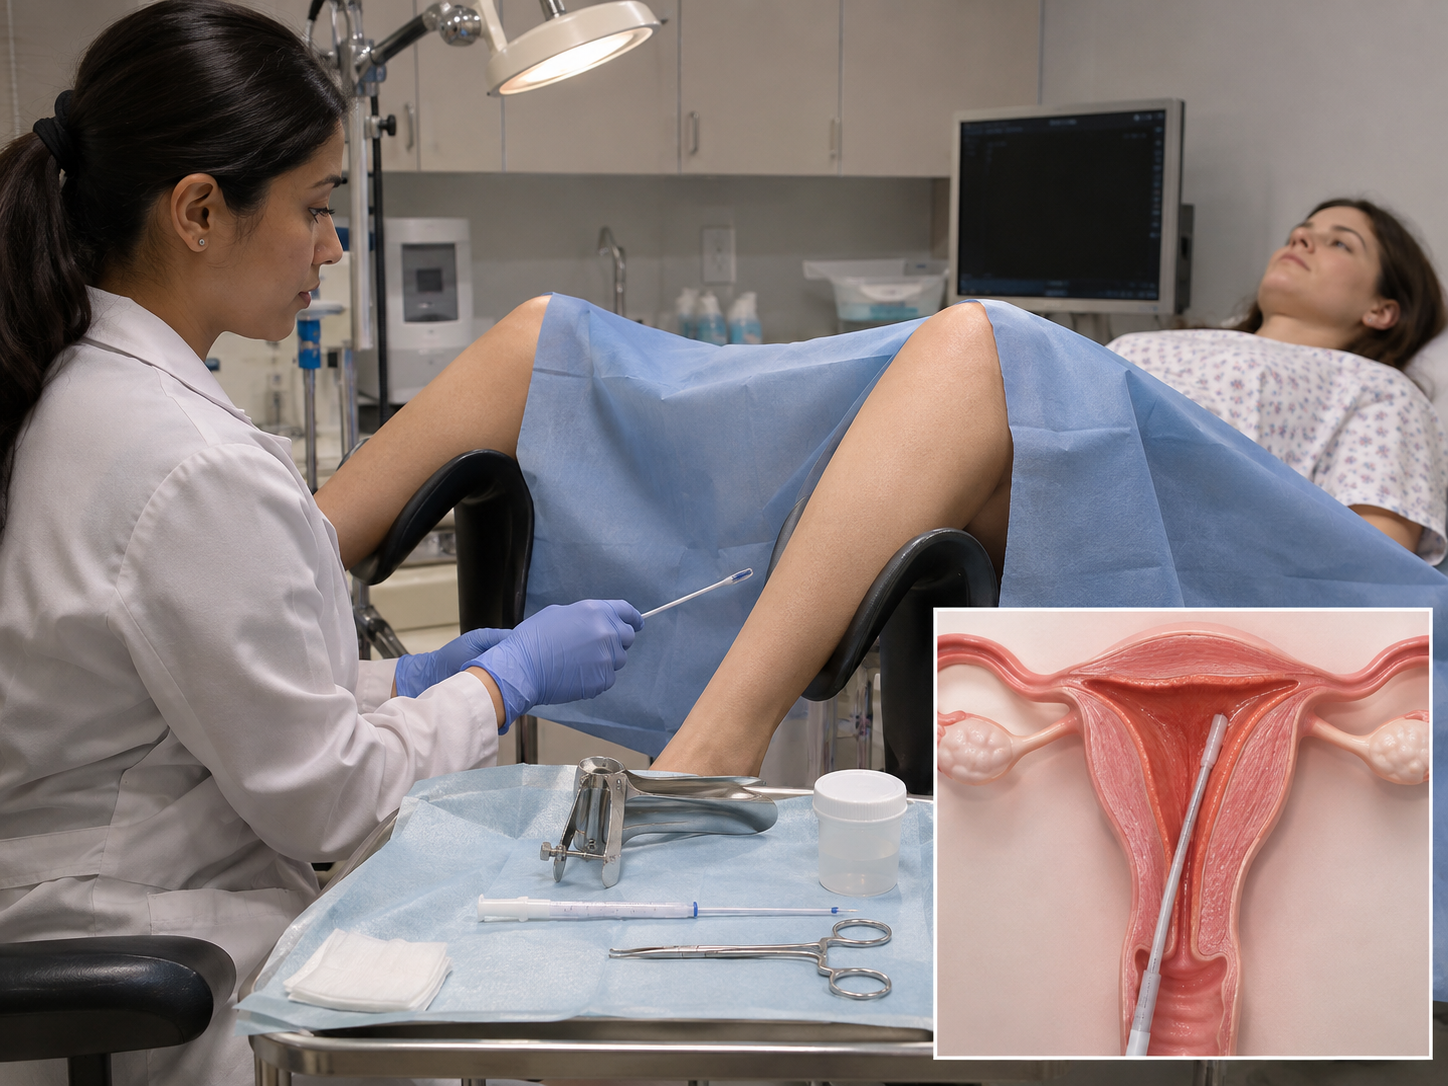
\includegraphics[width=0.82\textwidth]{images/chapters/procedure_endometrial_biopsy_overview.png}
\captionof{figure}{Endometrial Biopsy: A clinician collects a uterine-lining sample during an office examination.}
\end{minipage}
\end{center}
\section*{Common Instruments and Equipment}
The exact setup varies by technique and setting. Common items may include:
\begin{itemize}[nosep,leftmargin=*]
  \item endometrial sampling catheter or suction device
  \item speculum and tenaculum when needed
  \item specimen container and pregnancy test when appropriate
\end{itemize}

\section*{Alternative Names}
Endometrial sampling; uterine lining biopsy; Pipelle biopsy (a common office method).

\section*{Principle}
A clinician passes a thin sampling tube through the cervix into the uterus. Suction and gentle movement collect tissue from the lining. Other methods include sampling during hysteroscopy, when a small camera lets the clinician look inside the uterus and target an area.

\section*{History}
Dilation and curettage (D\&C) under anesthesia was once commonly used to obtain uterine tissue. Flexible suction devices made it possible to collect samples in many cases during an office visit. D\&C and hysteroscopy remain options when office sampling is unsuccessful, unsuitable, or more detailed assessment is needed.

\section*{Why It Is Done}
Common reasons include abnormal bleeding between periods, unusually heavy or prolonged periods, bleeding after menopause, or an ultrasound finding that needs tissue assessment. A clinician may also recommend sampling when a person has risk factors for endometrial overgrowth or cancer, or when bleeding continues despite treatment. It is a diagnostic test, not a routine screening test for people without symptoms.

\section*{Role in Care}
It is one of several tests used to investigate abnormal uterine bleeding. Whether it is appropriate depends on the person's age, symptoms, risk factors, examination, and imaging. For example, U.S. guidance commonly recommends sampling as a first-line test for abnormal uterine bleeding from age 45; younger people may need it when bleeding persists, treatment has not worked, or risk factors are present. For postmenopausal bleeding, 2026 ACOG guidance recommends both transvaginal ultrasound and tissue sampling as part of the initial evaluation for most patients. Guidance differs by country and indication: for heavy menstrual bleeding, NICE recommends taking a biopsy during hysteroscopy in selected higher-risk patients and advises against blind biopsy. Ultrasound, hysteroscopy, or other tests may be needed as well.

\section*{How It Is Performed}
The office procedure usually takes a few minutes. The patient lies on an examination table with feet supported. A speculum is placed in the vagina so the clinician can see the cervix, which may be cleaned. A narrow flexible tube is passed through the cervix into the uterus, and gentle suction collects tissue. Some people feel brief, strong menstrual-like cramps. Pain can be significant, so discuss pain-control options before the procedure. Depending on the person and setting, options may include an anti-inflammatory pain medicine or topical or injected local anesthetic. Sedation or anesthesia in another setting may also be discussed when appropriate and available. The patient can ask the clinician to pause or stop. The sample is sent to a laboratory.

If the cervix is difficult to pass, the sample is too small, or a focal area needs examination, the clinician may recommend another attempt, ultrasound guidance, hysteroscopy with a targeted biopsy, or sampling under anesthesia.

\section*{Preparation}
Follow the clinic's instructions. Tell the clinician if pregnancy is possible, if you have an infection or unusual discharge, if you take blood-thinning medicines, or if you have allergies or a history of difficult or painful pelvic procedures. A pregnancy test may be done when relevant because the procedure should not be performed during an ongoing pregnancy. Ask whether to take pain medicine beforehand and whether your regular medicines should be changed; do not stop prescribed medicines without advice.

\section*{Contraindications}
No specific absolute contraindication is identified here; the treating team assesses suitability for the individual.

\section*{Precautions}
An ongoing pregnancy is a reason not to perform routine endometrial sampling. A suspected pelvic or cervical infection usually needs assessment and treatment first. Cervical narrowing, uterine shape, bleeding, medicines that affect clotting, and prior procedures may affect whether or how the biopsy can be done. The clinician weighs these factors and may choose another method.

\section*{Risks}
Temporary cramping and light vaginal bleeding or spotting are common. Some people feel faint or nauseated. Less common complications include infection, heavier or prolonged bleeding, and a small hole in the uterus (perforation). A sample may be insufficient for diagnosis, and a blind sample can miss a localized problem such as a polyp or other focal lesion.

\section*{Aftercare and Recovery}
Most people return to usual activities the same day, but cramping or light spotting can continue for a short time. Use a pad if preferred and follow the clinic's advice about pain relief and when to resume sex, tampons, or other activities; instructions vary. Contact the clinic if you are unsure what is expected for you.

\section*{Outcome and Follow-up}
The pathology report may describe a normal pattern for the menstrual cycle, a thin or inactive lining, inflammation, hyperplasia, atypical cells, cancer, or tissue that is insufficient to interpret. The meaning depends on menstrual status, medicines, symptoms, and the reason for testing. The clinician explains the result and whether treatment or further evaluation is needed.

\section*{Expected Results}
A benign result means no abnormality was found in the tissue sampled. It does not always exclude a focal lesion or explain ongoing bleeding. An insufficient or failed sample is not the same as a reassuring normal result; the next step depends on symptoms, imaging, and individual risk.

\section*{Follow-up}
Review the result with the ordering clinician. Further testing, such as ultrasound or hysteroscopy with directed biopsy, may be needed if the sample is insufficient, imaging is abnormal, or bleeding persists or returns despite a benign result. Any bleeding after menopause should be discussed with a clinician, including when an earlier biopsy was normal.

\section*{When to Seek Medical Care}
Contact the clinic promptly for fever or chills, foul-smelling discharge, worsening pelvic pain, or bleeding that is heavier or lasts longer than the clinic said to expect. Seek urgent care for severe pain, very heavy bleeding, fainting, or rapidly worsening symptoms.

\section*{References}
\begin{enumerate}
  \item American College of Obstetricians and Gynecologists. Abnormal Uterine Bleeding. https://www.acog.org/womens-health/faqs/abnormal-uterine-bleeding
  \item American Academy of Family Physicians. Endometrial Biopsy: Tips and Pitfalls. https://www.aafp.org/pubs/afp/issues/2020/0501/p551.html
  \item East Kent Hospitals University NHS Foundation Trust. Endometrial Pipelle Biopsy. https://leaflets.ekhuft.nhs.uk/endometrial-pipelle-biopsy/html/
  \item American College of Obstetricians and Gynecologists. Updated Guidance Regarding the Role of Transvaginal Ultrasonography in Evaluating the Endometrium of Individuals With Postmenopausal Bleeding. Clinical Practice Update; 2026. https://doi.org/10.1097/aog.0000000000006275
  \item American College of Obstetricians and Gynecologists. Pain Management for In-Office Uterine and Cervical Procedures. https://www.acog.org/clinical/clinical-guidance/clinical-consensus/articles/2025/05/pain-management-for-in-office-uterine-and-cervical-procedures
\end{enumerate}

\clearpage
